\documentclass[aps,prc,reprint,amsmath,nofootinbib]{revtex4-1}

\usepackage{hyperref}
\usepackage{graphicx}
\usepackage{subcaption}
\usepackage{tabularx}
\graphicspath{{fig/}}

%\usepackage{tikz}
%\usetikzlibrary{shapes,calc,matrix}

%\usepackage{mdwlist}
%\renewcommand\labelitemi{\raisebox{.3ex}{\tiny$\bullet$}}

%\newcommand{\trento}{T\raisebox{-.5ex}{R}ENTo}
%\newcommand{\nch}{N_\text{ch}}
%\newcommand{\eccratio}{\sqrt{\langle \varepsilon_2^2 \rangle}/\sqrt{\langle \varepsilon_3^2 \rangle}^{\,0.6}}

\begin{document}

\title{Entropy deposition in ultra-relativisitic nucleus-nucleus collisions}

\author{J.\ Scott Moreland}
\date{\today}

\maketitle

\section{Introduction}

Microseconds after the big bang, our universe was super heated to several trillion kelvin. In these extreme conditions, nuclear matter existed as a hot 
soup of deconfined quarks and gluons. As the universe expanded and cooled, these colored degrees of freedom recombined to 
form colorless hadrons (e.g. protons) and kickstarted the elaborate process of nucleosysnthesis \cite{Heinz:2004qz}.

Evidence for this high temperature phase of deconfined nuclear matter was provided by researchers at the Relativisitic Heavy-Ion Collider (RHIC) 
in Brookhaven, NY. Collisions of ultra-relativistic gold nuclei at RHIC produced hot and dense fireballs that exhibited strong signs of collective flow 
\cite{Adams:2005dq}. These flow results were significantly stronger than those of lower energy nuclear collisions at the Super Proton Synchrotron (SPS) 
\cite{Shuryak:2004cy}. This energy dependent growth in collectivity led RHIC scientists to announce indirect evidence for a new state of deconfined nuclear 
matter dubbed the quark-gluon plasma (QGP) \cite{BNL}.

The large flow signals observed at RHIC supported a \emph{strongly} coupled QGP liquid and upended wide expectations that high temperature nuclear matter 
would exhibit small coupling $\alpha_s(p~T) \ll 1$ and behave like a weakly interacting gas \cite{Shuryak:2004cy}. Relativistic fluid dynamic simulations which modeled 
the produced fireball using distinct liquid and gaseous phases to describe the strongly coupled QGP liquid and weakly coupled hadron gas were highly successful in 
explaining the anomalous flow behaviour observed in the data and established the hydrodynamic nature of hot and dense nuclear matter \cite{Kolb:2003dz}.

The success of these first hydrodynamic simulations, which did not account for viscosity, suggested that the QGP was nearly inviscid. In fact, ideal hydrodynamics 
worked so well in describing the evolution of relativistic heavy-ion collisions that the QGP was called the ``perfect fluid''. It has since become a task of great 
interest to extract the thermodynamic and transport properties of the QGP droplet produced in relativistic heavy-ion collisions, as such properties shed light on
exotic regions of the nuclear phase diagram and improve our murky understanding of primordial matter in the big bang.

\subsection{Extracting QGP properties}

Fundamental QGP properties are extracted from computer simulations using a process known as model to data comparison. Theoretical guidance is used to construct
realistic, albeit under constrained, hydrodynamic models for the full spacetime evolution of the produced fireball. These models generate events exactly as they might
occur inside the detector and output moc experimental data. By comparing the model's moc data to experimental data, free parameters of the model are constrained. Such 
model to data comparisons thus provide valuable access to fundamental properties of the short lived QGP fireball which cools too quickly (${\sim}10^{-23}$ s) to be 
observed directly.

In order to extract these properties accurately, it's important that the model admit a faithful description of reality. In this report we concentrate on improving 
initial condition models used to describe the deposition of entropy in relativistic hydrodynamic simulations. The veracity of these initial conditions governs the 
predictive power of hydrodynamic model to data comparisons and consequently our understanding of fundamental QGP properties.
  
\section{Relativistic nuclear collisions}

Before talking about the specifics of hydrodynamic initial conditions and why they are important to QGP parameter extractions, it's useful to take a step back 
and discuss in detail the current picture of relativistic heavy-ion collisions. For reasons which become clear in the following sections, I drop the 
label ``heavy-ion'' and generalize the dicussion to arbitrary nucleus-nucleus collisions.

\subsection{Collision and rapid thermalization}

\begin{figure*}
  \centering
  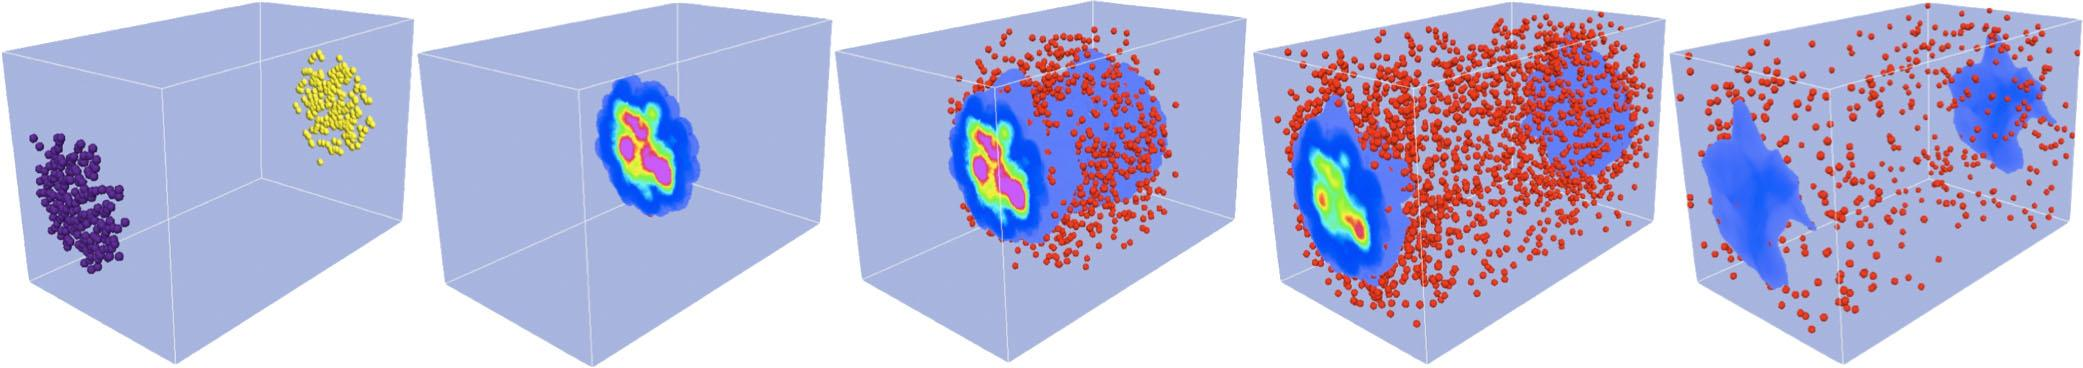
\includegraphics[width=\textwidth]{evolution} \\
  0 fm/c   \hspace{.13\textwidth}
  0.5 fm/c \hspace{.13\textwidth}
  8 fm/c   \hspace{.13\textwidth}
  16 fm/c  \hspace{.13\textwidth}
  22 fm/c
  \caption{Computer simulation of a gold-gold collision at $\sqrt{s}=200$ GeV. Projectile nucleus (purple) collides with target nucleus (yellow) and produces a QGP (heat map). 
  Red spheres indicate cooler hadron resonance gas. \cite{iss}.}
  \label{fig:evolution}
\end{figure*}

Consider as an example two nuclei with atomic mass numbers $A_1$ and $A_2$ which have been accelerated to $\beta=0.9999$ times the speed of light and travel towards
each other along an imaginary beam axis. When viewed from the laboratory frame, the nuclei are Lorentz contracted along the beam-axis by a Gamma-factor 
$\gamma \approx 70$ and thus appear highly compressed. 

In the rest frame of each nucleus, the nuclei are described by the multi-body nuclear wavefunctions $\Psi_{A_1}$ and $\Psi_{A_2}$ with normalization condition  
\begin{equation}
\int d\vec{x}_1 ... d\vec{x}_A \left | \Psi_A(\vec{x}_1,...,\vec{x}_A) \right|^2 = A.
\end{equation}

The act of collision collapses these wavefunctions and samples a discrete set of nucleon coordinates,
\begin{equation}
 \Psi_{A_1} \rightarrow \{\vec{x_1},...,\vec{x}_{A_1}\} ~~~~ \mbox{and} ~~~~ \Psi_{A_2} \rightarrow \{\vec{x_1},...,\vec{x}_{A_2}\}
\end{equation}
depicted\footnote{The simulation used to generate FIG. \ref{fig:evolution} admittedly resolves discrete nucleons before any collision has taken place.} in panel one 
of FIG. \ref{fig:evolution}. These nucleon configurations may either partially or fully overlap in the moment of collision allowing for various numbers of nucleon 
collisions in a single nucleus-nucleus collision. This first instant of impact defines the collision starting time $\tau=0$ fm/c in units of longitudinal proper time $\tau^2 = t^2-z^2$.

The struck or ``wounded'' nucleons which participate in the collision penetrate each other in the first fraction of a fm/c and liberate quarks and gluons described by 
their nuclear structure functions. These primary quarks and gluons generate secondary partons which are deposited in the plane transverse to the beam axis centered 
at the collision epicenter. The exact physical processes describing these early-time dynamics remain poorly understood and numerous theoretical models exist. We 
discuss two such models for initial particle production in section ?. 

The initial partonic fireball at incremental time $\tau=0^+$ fm/c is lumpy in the transverse plane and flattened along the beam axis. Transverse fluctuations in the 
density of produced partons reflect fluctuations in configurations of nucleons within the colliding nuclei. 

The secondary energetic partons quickly rescatter and reach thermal equillibrium if the interactions are sufficiently strong. Studies suggest that thermalization 
occurs rapidly in relativistic heavy-ion collisions and sets in around $\tau_{themal} \approx 0.6$ fm/c in $\sqrt{s} = 200$ GeV gold-gold collisions \cite{Heinz:2001xi}.

\subsection{Hydrodynamic evolution}

Once the system reaches thermalization, relativistic hydrodynamics can be used to evolve the thermalized state forward in time. The hydrodynamic equations of motion 
are a set of conservation equations which conserve the flow of four-momentum and net baryon current,
\begin{equation}
 \partial_\mu T^{\mu\nu} = 0 ~~~~~\mbox{and}~~~~~ \partial_\mu j_B^\mu = 0.
\end{equation}

In the ideal (inviscid) limit, the energy momentum tensor and net baryon current can be decomposed as,
\begin{eqnarray}
 \cr T^{\mu\nu} &=& (\varepsilon + p) u^\mu u^\nu - p g^{\mu\nu} \\
 j_B^\mu &=& n u^\mu
\end{eqnarray}
where $\varepsilon$ denotes the system's energy density, $p$ the pressure, $u^\mu$ the fluid four-velocity, $n$ the local baryon density and $g^{\mu\nu}$ the metric 
tensor.

Altogether we are left with $5$ equations of motion to describe $6$ field quantities ($\varepsilon$, $p$, $u^1$, $u^2$, $u^3$ and $n$).
The system of equations is closed by adding an additional thermodynamic relation between two of the thermal field quantities, e.g. energy density and pressure. 
This additional relation is known as the equation of state (EOS).

Quite conveniently, the EOS of high temperature, thermal QCD is directly calculable from the QCD Lagrangian using the method of Lattice QCD. The partition function
is expressed in terms of the vaccuum to vaccuum transition amplitude of quark and gluon fields in the Feynman path integral formalism and solved numerically on a
discrete grid. Once the partition function is known, the energy density, entropy density, pressure and temperature are easily interrelated. 

This high temperature EOS is used to model hot and dense regions of the fireball above the critical QGP phase transition temperature $T_c$. At low temperatures,
the QGP EOS is matched to a hadron resonance gas EOS which describes the fluid dynamic behaviour of the QGP once it hadronize into a dillute gas of bound quark
states. In this manner, the hydrodynamic model naturally describes the complicated dynamics of hadronization which are extremely difficult to model microscopically.

\subsection{Transition to Boltzmann transport}

\begin{figure*}
 \includegraphics[height=0.2\textwidth]{collision1}
 \includegraphics[height=0.2\textwidth]{collision2}
 \includegraphics[height=0.2\textwidth]{collision3}
 \includegraphics[height=0.2\textwidth]{collision4}
 \caption{\label{fig:spacetime}}
\end{figure*}

As the system evolves hydrodynamically it expands and cools. The low temperature system eventually becomes that of a hadron resonance gas. While the QGP is a 
roughly homogenous mixture of quarks and gluons, the hadron resonance gas is a complicated, heterogeneous mixture of hadrons and hadronic resonances. Inelastic collisions 
amongst these particles alter the system's chemical composition and drive the system away from chemical equillibirum. 

For these reasons, it is common to switch from hydrodynamics to a Boltzmann description below the QGP phase transition temperature $T_c$. Boltzmann dynamics naturally 
incorporate chemical nonequillibrium and allow for a more detailed description of the system's low temperature evolution.

To switch from hydrodynamic fields to discrete molecular dynamics, the hydrodynamic medium is first ``particleized''. Particles are sampled from the Cooper-Frye formula 
which describes the particle spectra along a freeze-out hypersurface of constant temperature,
\begin{equation}
 \label{cooper_frye}
 E \frac{dN_i}{d^3p} = \int_\sigma f_i(x,p) p^\mu d^3\sigma_\mu.
\end{equation}
In equation \ref{cooper_frye}, $f_i$ is the particle distribution function, $p^\mu$ is the local fluid four-momentum and $d^3\sigma_\mu$ characterizes an element of the freezeout hypersurface. Equation
\ref{cooper_frye} is integrated over the full freezeout hypersurface to sample particles from the fluid which are then piped into Boltzmann transport simulations.

The Boltzmann equation simulates all elastic and inelastic collisions between the sampled particles until the system becomes too dillute to continue interacting. In symbollic
form it can be written as,
\begin{equation}
 \label{boltzmann_eqn}
 \frac{df_i(x,p)}{dt} = \mathcal{C}_i (x,p),
\end{equation}
where $f_i(x,p)$ is the distribution function of the $i^\mathrm{th}$ particle species and $\mathcal{C}_i$ is the corresponding collision kernel which describes all source 
terms in a collision.

After the particles finish interacting, their positions, momenta and particle ID's are recorded and stored to file. This moc experimental data is then compared with real
data, and free parameters of the model are tuned to optimally replicate reality. The quantities of interest in such a procedure are thus under constrained parameters of 
the model. 

In the next section, I talk about one such quantity, the hydrodynamic specific shear viscosity $\eta/s$ which arises from dissipative corrections to ideal hydrodynamics.
Model to data extractions of $\eta/s$ indicate that the shear viscosity of the QGP is astonishingly small. Current estimates of the QGP shear viscosity place bounds $0.08 \le \eta/s \le 0.20$. For comparison, the values of $\eta/s$ 
for water at room temperature are $\eta/s \approx 30$. The QGP has consequently been called the ``perfect fluid''. We discuss current methods for extracting $\eta/s$ from
model to data comparisons and isolate the largest source of uncertainty in these extractions.

\section{Constraining the QGP viscosity}

When a nuclear collision is viewed along the beam axis, the nuclei collide and overlap in the plane orthogonal to the beam axis, offset by a random separation vector $b$ 
(see FIG. 1a). The resulting almond shaped fireball is highly anisotropic and is described by energy density gradients which are larger along its short axis. These larger 
energy density gradients generate larger pressure gradients and hence drive more flow. Consequently, the system flows faster along the short axis and g

Additional fluctuations in the distribution of nucleons within each nucleus distort the almond shape of the produced fireball. These fluctuations are uncorrelated with the 
impact parameter geometry of the collision and hence cannot be characterized by a single elliptic shape. For example, it's entirely possible that random nucleon fluctuations
generate a triangular fireball with corresponding triangular flow profile (FIG. 1b). 

It's worth stressing that this conversion from spatial anisotropy to flow anisotropy is a characteristic signature of hydrodynamic behaviour. The efficiency of conversion
tells us about the strength of dissipative forces in the fluid, most notably the fluid viscosity.

\subsection{Viscosity from anisotropic flow}

Hydrodynamic conversion from spatial anisotropy to momentum anisotropy becomes easier to quantify if we first decompose the initial and final states using an azimuthal 
Fourier expansion. 

The initial state spatial anisotropy is characterized by the Fourier eccentricity harmonics $\varepsilon_n$ given by,
\begin{equation}
 \varepsilon_n e^{-i n \Phi_n} = -\frac{\int dx\,dy\,r^n e^{i n \phi} s(x,y)}{\int dx\,dy\, r^n s(x,y)}
\end{equation}
where $n$ denotes the eccentrcity harmonic mode number, $\Phi_n$ denotes the direction of the steepest density gradient and $s(x,y)$ the event's transverse entropy density
(often energy is used as well). Examples of eccentricity harmonics two, three, four and five are shown in FIG. \ref{fig:harmonics}.

An analogous expansion for the final state flow anisotropy yields the flow coefficients $v_n$,
\begin{equation}
 v_n(y) e^{i n \Psi_n(y)} = \frac{\int p_T dp_T d\phi_p e^{i n \phi_p} \frac{dN}{dy p_T dp_T d\phi_p}}{\int p_T dp_T d\phi_p \frac{dN}{dy p_T dp_T d\phi_p}}
\end{equation}
where $n$ denotes the anisotropic flow mode number, $\Psi_n$ denotes the angle of maximum flow, $p_T$ a particle's transverse momentum and 
$y=\tfrac{1}{2}\log(\tfrac{E+p_z}{E-p_z})$ its rapidity.

Hydrodynamic expansion converts n-th order eccentricity $\varepsilon_n$ into n-th order harmonic flow $v_n$ with a conversion efficiency that's proportional to the fluid's
specific shear viscosity $\eta/s$,
\begin{equation}
 \label{linear_response}
 v_n \propto \eta/s \cdot \varepsilon_n.
\end{equation}

Thus \emph{if} one possessed a realistic initial condition model from which they could calculate the eccentricity harmonics $\varepsilon_n$, \emph{and} they had faith 
in their hydrodynamic description of the produced plasma, \emph{then} they could calculate the flow harmonics $v_n$ from equation \ref{linear_response} for different values 
of the QGP viscosity and find the one which optimally fits experimental flow measurements.

Somewhat surprisingly, the biggest obstacle in this whole procedure is not the derivation of relativistic viscous hydrodynamics, or calculations of the lattice equation
of state or even microscopic descriptions of the hadron resonance gas - it's a description of the system's hydrodynamic initial conditions. 

\begin{figure}[t]
 \includegraphics[width=0.15\columnwidth]{e2-crop} \hspace{.01\columnwidth} 
 \includegraphics[width=0.23\columnwidth]{e3-crop} \hspace{.01\columnwidth}
 \includegraphics[width=0.21\columnwidth]{e4-crop} \hspace{.01\columnwidth}
 \includegraphics[width=0.24\columnwidth]{e5-crop}\\
 \flushleft
 \vspace{-0.1in}
 \hspace{0.08\columnwidth} 2 \hspace{0.19\columnwidth} 3 \hspace{0.21\columnwidth} 4 \hspace{0.22\columnwidth} 5
 \caption{\label{fig:harmonics} Diagrams of the second, third, fourth and fifth azimuthal Fourier harmonics. The angular resolution increases with increasing harmonic number.}
\end{figure}

\section{Initial condition models}

Hydrodynamic initial conditions describe the thermal state of the QGP fluid at the QGP thermalization time $\tau_{therm} \approx 0.6$ fm/c. These initial condition models
fall into two general categories - dynamical models which calculate the initial state of the system at time $\tau=0$ fm/c and explicitly simulate the pre-equillibrium 
dynamics which drive the system to thermalization, and effective models which omit early-time dynamics to generate profiles of energy or entropy \emph{at} the QGP thermalization time. 
Historically, effective models have been preferred for their simplicity, and despite recent advances in pre-equillibirum transport theory, remain the most popular.

\subsection{Glauber modeling}

The most famous effective model for hydrodynamic initial conditions is the well known Glauber model. The Glauber model asserts that particle production in nucleus-nucleus 
collisions scales with a linear combination of ``hard'' and ``soft'' collision processes. 

For hard processes, it's natural to assume that the number of produced particles scales with the number of binary nucleon-nucleon collisions. Hard processes correspond
to large momentum transfer and are well localized in the collision. This means that interference effects can be safely ignored. In contrast, soft processes correspond to low 
momentum transfer and hence long wavelengths. These soft collisions are strongly affected by coherence effects and should not scale linearly with the number of
binary collisions.

Soft processes are particularly challenging because they are inherently non-perturbative (strong coupling) and thus cannot be calculated using the usual tools
of perturbative QCD. The Glauber model thus adopts an ansatz for soft particle production and scales soft processes with the number of wounded nucleons, i.e. nucleons 
which participate in at least one collision. In this picture, successive nucleon collisions change the excited state of the wounded nucleon but do not contribute to 
overall particle production. The excited nucleons become de-excited once they leave the interaction region and thus generate secondary densities proportional to the 
initial density of wounded nucleons.

Binary collisions and wounded nucleons are typically counted by considering all possible pairs of nucleon-nucleon collisions which occur with probability
\begin{equation}
P_{coll}=
\begin{cases}
  1 &\mbox{if } b \le \sqrt{\sigma^{inel}_{NN}/\pi} \\ 
  0 &\mbox{if } b > \sqrt{\sigma^{inel}_{NN}/\pi},
\end{cases}
\end{equation}
where $b$ denotes the nucleon-nucleon impact parameter and $\sigma^{inel}_{NN}$ the inelastic nucleon-nucleon cross section.

These particle interactions are then converted to smooth density profiles by depositing a small Gaussian about each wounded nucleon coordinate and binary
collision vertex. The resulting density profiles are then projected onto the transverse plane yielding,
\begin{eqnarray}
 \label{BC_WN}
 \cr BC(x,y) &=& \sum_{i=1}^{N_{coll}} \frac{1}{\sqrt{2 \pi \sigma^2}} e^{ -|\vec{r}_\perp-\vec{r}_{i\perp}|^2/2 \sigma^2 }   \\
 WN(x,y) &=& \sum_{i=1}^{N_{part}} \frac{1}{\sqrt{2 \pi \sigma^2}} e^{ -|\vec{r}_\perp-\vec{r}_{i\perp}|^2/2 \sigma^2 } .
\end{eqnarray}
where the Gaussian deposition width $\sigma$ is a free parameter.

The entropy (or often energy) density of the fireball is finally set proportional to a linear combination of the binary collision and wounded nucleon densities,
\begin{equation}
 \frac{dS(x,y)}{d^2r_\perp dy} \propto \frac{1-\alpha}{2} WN(x,y) + \alpha\, BC(x,y),
\end{equation}
where $dS(x,y)/d^2r_\perp dy$ is the fireball's transverse entropy density, $\alpha$ is a unitless tunable parameter and $\vec{r}_\perp$ is a position in the 
transverse plane. We note that the Glauber model projects all densities onto the transverse plane and thus does not resolve any structure along the collision beam axis.

\subsection{Color-Glass Condensate theory}

In Color-Glass Condensate theory, the transverse entropy density at mid-rapidity scales with the density of secondary gluons produced by individual gluon-gluon interactions.
This density depends on the number of available states, and in turn on the local gluon distribution functions in each colliding nucleon pair. These gluon distribution 
functions are connected to the underlying nuclear geometry through a parameter known as the saturation scale $Q_s$ via it's dependence on the nuclear thickness 
functions $T_{A_1}$ and $T_{A_2}$ which describe the transverse opacity of participant nucleons in each nucleus,
\begin{equation}
 \label{thickness}
 T_A(x,y) = \sum\limits_{i=1}^{A} \frac{1}{\sqrt{2 \pi \sigma^2_p}} e^{ -|\vec{r}_\perp-\vec{r}_{i\perp}|^2/2 \sigma_{p}^2 }.  
\end{equation}
We note that the nuclear thickness function defined in equation \ref{thickness} is indentical to the wounded nucleon density in equation \ref{BC_WN}, except that the 
summation runs over nucleons in a single nucleus with Gaussian width $\sigma_{p}$ given by the proton charge radius.

There exist a number of Color-Glass Condensate realizations which convert the nuclear thickness functions $T_{A_1}$ and $T_{A_2}$ defined by equation \ref{thickness} into 
secondary gluon densities and hence entropy densities at mid-rapidity, but we only discuss one for the sake of brevity.

The Kharzeev-Levin-Nardi (KLN) model is one well known implementation of Color-Glass Condensate effective field theory. In the KLN model, the gluon saturation scale 
$Q_s$ is parameterized by
\begin{equation}
 Q^2_s(x;{\bf r}_\perp) = 2\, \mbox{GeV}^2 \left( \frac{T({\bf r}_\perp)}{T_0} \right) \bigg( \frac{x_0}{x} \bigg)^\lambda,
\end{equation}
where $T_0=1.53$ fm$^{-2}$ and $x_0 = 0.01$. Here $x=p_\perp \exp(\pm y)/\sqrt{s}$ is the light-cone momentum fraction of a gluon and $\lambda$ is a 
dimensionless parameter tuned to fit the observed hadron multiplicity in central collisions.
 
The gluon distribution functions are then expressed in terms of the gluon saturation scale as,
\begin{equation}
 \phi(x,k^2_\perp,{\bf r}_\perp) \sim \frac{1}{\alpha_s(Q_s^2)}\frac{Q_s^2}{\max(Q_s^2,k_\perp^2)}
\end{equation}
where $k_\perp$ is the transverse momentum of a gluon and $\alpha_s$ specifies the strength of the coupling constant. 

Once the gluon distribution functions are known, the density of produced gluons is calculated by integrating a gluon fusion term over the full collision phase space,
\begin{eqnarray}
 \cr \frac{dN_g}{d^2r_\perp dy} &=& \frac{2 \pi^2}{C_F} \int^{p_\perp^{max}} \frac{d^2 p_\perp}{p_\perp^2} \int^{p_\perp} \frac{d^2 k_\perp}{4} \alpha_s(Q_s^2) \\
 &\times& \phi_1(x_1,({\bf p}_\perp + {\bf k}_\perp)^2/4; {\bf r}_\perp) \\
 &\times& \phi_2(x_2,({\bf p}_\perp - {\bf k}_\perp)^2/4; {\bf r}_\perp),
\end{eqnarray}
where $C_F$ is a color factor, $\phi_1$ and $\phi_2$ are the gluon distribution functions of each nucleus and $p_\perp = p_\perp^1 + p_\perp^2$ and 
$k_\perp = p_\perp^1 - p_\perp^2$ denote the primary transverse gluon momentum in center of mass coordinates. This furnishes the transverse entropy density up to an 
overall normalization factor,
\begin{equation}
 \frac{dS(x,y)}{d^2r_\perp dy} \propto \frac{dN_g}{d^2r_\perp dy}.
\end{equation}

\section{The case for new I.C. models}

Originally, collective flow behaviour was thought to only exists in collisions of \emph{heavy} nuclei where the produced fireball is sufficiently large and dense to reach 
a state of local thermal equillibrium. Proton-lead collisions, on the other hand, were thought to be too small to produce any signatures of collective flow.

It thus came as a great surprise when proton-lead collisions - which were scheduled primarily as a calibration run for larger collisions - produced significant signs of 
collective behaviour. This discovery raised several key questions within the heavy-ion community:
\begin{itemize}
 \item Do small collision systems produce a QGP? 
 \item Are the hydrodynamic equations of motion valid in small systems?
 \item If so, how do we unite large and small systems under a single theoretical framework?
\end{itemize}

The application of the Glauber and KLN models to the full range of collision systems measured at RHIC and the LHC has been carried out with mixed success. The KLN model
struggles to replicate the full spectrum of measured anisotropic flow coefficients and the Glauber model has problems describing collisions of deformed nuclei, while 
both models do a poor job describing small collision systems. There is in fact only one model, a CGC derivative called IP-Glasma, which has provided an excellent 
description of flow harmonics in heavy nuclei at RHIC and the LHC, but even its application to smaller collision systems remains uncertain.

Perhaps even more worrisome than flow inconsistencies, which may simply result from applying hydrodynamics where it's not applicable, are inconsistencies in the description 
of particle production; there are models which provide satisfactory descriptions of particle production in proton-proton collisions, and there models which provide 
satisfactory descriptions of particle production in heavy-ion collisions, but very few models do both simultaneously. 

Yet if we look at the density of nuclear overlap in heavy-ion collisions, we see that there are regions of overlap which are identical to those found in light-nucleus 
collisions. For example, isolated proton-proton collisions frequently occur around the edges of gold-gold collisions. In fact, a wide range of $n$-on-$m$ nucleon-nucleon 
collisions occur \emph{inside} a single heavy-ion collision. It's thus hard to trust any model which claims to simulate the overall distribution of matter in large nucleus-nucleus collisions without simulatenously describing the 
distribution of matter produced by all collision sub-fragments. 

\section{Particle production as a mapping}

\begin{figure}
 \includegraphics[height=0.19\textwidth]{motivation1-crop}\\
 \caption{\label{fig:motivation_beam} Beam view: imaginary Cartesian grid superimposed on top of nuclear overlap region}
 \includegraphics[height=0.13\textwidth]{motivation2-crop}
 \caption{\label{fig:motivation_side} Side view: Example of a grid cell containing a localized three-on-two nucleon collision}
\end{figure}

We now firm up the motivation for a composite description of the QGP fireball with a heuristic argument. Imagine that we have the freedom to construct and collide any 
$m$-on-$n$ combination of $m$ projectile and $n$ target nucleons. The experiment is performed and the average number of charged particles in a fixed 
interval about mid-rapidity recorded,
\begin{equation}
 \label{charged_particles}
 N_{ch}(|\eta|<\eta_{max};\, n,\, m).
\end{equation}

For example, the simplest combination of projectile and target nucleons is a $1$-on-$1$ collision of two protons,
\begin{equation}
 N_{ch}(|\eta|<1;\, 1,\, 1).
\end{equation}
A single proton is then added to the target nucleus, positioned just behind the original target proton in line with the beam axis, and the collision is repeated at the 
same beam energy yielding a new measurement for a $1$-on-$2$ collision,
\begin{equation}
 N_{ch}(|\eta|<1;\, 1,\, 2).
\end{equation}

At this point you can probably see where we are headed. We continue to extend the projectile and target nuclei by adding  protons to the column of existing protons 
and record the number of charged particles measured in the collision. We thus build up a two dimensional surface that describes particle production for any $m$-on-$n$ 
collision. We will now argue that this surface is all we need to approximate entropy deposition in the early stages of a generic nucleus-nucleus collision. 

\section{Reverse engineering the fireball}

Hybid hydrodynamic + Boltzmann transport simulations indicate that, to good approximation, the simulation's initial entropy is a close proxy for final state particle 
production \cite{Heinz}. This linear correspondence is of course affected by small corrections from viscous entropy production and inelastic collisions in the hadron 
resonance gas, but nevertheless holds quite well. 

We use this linear relation to revert equation \ref{charged_particles} into a statement about initial entropy deposition,
\begin{equation}
 \label{entropy_mapping}
 N_{ch}(|\eta|<1;\, n,\, m) \propto S(|\eta|<1;\, n,\, m),
\end{equation}
where $S$ is the initial entropy deposited in the rapidity interval $|\eta|<1$ by an $m$-on-$n$ collision. 

We now imagine a realistic collision of two heavy nuclei which overlap at some non-zero impact parameter in the transverse plane. We can superimpose an imaginary
Cartesian grid on top of this overlap region and model each grid cell as an $m$-on-$n$ collision of projectile and target nucleons 
(see FIG. \ref{fig:motivation_beam}, \ref{fig:motivation_side}). We can then simply read off the value of entropy deposition from equation \ref{entropy_mapping} 
for each grid cell and renormalize the entire profile to account for the unknown entropy to particle number conversion factor.

Unfortunately, nature will not allow us to construct elongated stacks of protons or even control the orrientation of nuclei when they collide. Therefore we cannot simply
measure particle production for every possible $m$-on-$n$ collision. Instead, we start from a suitably flexible ansatz for entropy deposition and constrain our ansatz 
using the full gamut of nucleus-nucleus multiplicity data.

\subsection{Ansatz for entropy deposition}

In our original line of reasoning, we formulated the problem in terms of global quantities such as the \emph{number} of nucleons in the projectile and target.
We can easily recast expression \ref{entropy_mapping} locally by replacing nucleon number with nuclear density,
\begin{equation}
 \frac{dN_{ch}}{d\eta} \propto \frac{dS}{d\eta} \bigg|_{\tau=\tau_0} \propto f(T_A,T_B)
\end{equation}
where $T_A$ and $T_B$ are the beam-integrated nuclear densities defined in equation \ref{thickness}.

We insist that the mapping $f$ respect several key properties,

\begin{figure}
 \includegraphics[width=\columnwidth]{saturation}
\end{figure}

\begin{figure}
 \includegraphics[width=\columnwidth]{trento-profiles}
\end{figure}

\begin{figure*}
 \includegraphics[width=\textwidth]{multdist}
\end{figure*}

\begin{figure*}
 \includegraphics[width=\textwidth]{eccentricity}
\end{figure*}

\bibliography{prelim,duke-qcd-refs/Duke_QCD_refs}


\end{document}
